\section{Computational Viability}
\label{sec:Results_Computational}

The computational viability of the \ac{eco-glosa} and \ac{flow-glosa} algorithms was assessed through the \ac{traci} interface to \ac{sumo}. Because absolute execution times depend on hardware, operating‐system specifics and background load, the discussion below focuses on \textit{relative} overheads. Tables~\ref{tab:CompViability_TraciComparison} and \ref{tab:CompViability_SumoTraci} list the raw durations for traffic volumes between $69$ and $3462\,\mathrm{veh/h}$.
\mynewline
Across every demand level and for both fuel models, \ac{eco-glosa} is markedly slower than \ac{flow-glosa}. At the lowest demand of $69\,\mathrm{veh/h}$, Table~\ref{tab:CompViability_TraciComparison} shows almost identical runtimes at $0\%$ \ac{mpr}, $18.64$ s for \ac{eco-glosa} and $18.89$ s for the baseline because neither algorithm performs optimisation when no vehicle is equipped. By contrast, at $100\%$ \ac{mpr} the baseline finishes in $154.27$ s, whereas \ac{eco-glosa} needs $282.56$ s, i.e.\ an $83\%$ increase. The disparity widens with the more demanding PHEMlight5 model: $19.74$ s (Standard) versus $954.95$ s (\ac{eco-glosa}) at full penetration, giving a slowdown of $\frac{954.95}{19.74}\approx 48.4\times$. The additional cost is attributable to the fuel-minimisation routine that \ac{eco-glosa} evaluates for every equipped vehicle at each simulation step, together with the finer transient resolution of PHEMlight5 that multiplies the number of engine-map look-ups.
\mynewline
Performance gaps grow super-linearly with traffic volume. Under HBEFA4 and $3462\,\mathrm{veh/h}$, the \ac{flow-glosa} requires $7\,670.32$ s at $100\%$ \ac{mpr}, while \ac{eco-glosa} takes $64\,860.61$ s, an $8.46\times$ overhead. PHEMlight5 accentuates the penalty: $7\,713.73$ s (\ac{flow-glosa}) versus $251\,661.36$ s (\ac{eco-glosa}), corresponding to a $32.6\times$ slowdown. At volumes beyond $3000\,\mathrm{veh/h}$, therefore, a \ac{traci}-based \ac{eco-glosa} study can become computationally prohibitive unless parallelisation or a native C++ plug-in is employed.
\mynewline
Interface choice is an additional bottleneck. Table~\ref{tab:CompViability_SumoTraci} compares native \ac{sumo} with the \ac{traci} client–server protocol for \ac{flow-glosa}. For $69\,\mathrm{veh/h}$ the \ac{traci} run takes $138.50$ s at $90\%$ \ac{mpr}, whereas native \ac{sumo} completes the same scenario in $15.31$ s, \enquote{a nine-fold overhead} caused by per-step socket communication and XML parsing. In the saturated regime of $3462\,\mathrm{veh/h}$ and $10\%$ \ac{mpr}, \ac{traci} requires $3029.19$\,s versus $738.94$\,s in native \ac{sumo}, a $4.10\times$ overhead. At $60\%$ \ac{mpr} the penalty grows to $12.13\times$ (with $8613.54$\,s vs.\ $709.81$\,s), demonstrating that \ac{traci} communication overhead is substantial even at low optimisation loads.  
\mynewline
Figure~\ref{fig:Comp_69} visualises the low-demand behaviour. Figure~\ref{fig:Comp_69_HBEFA4} shows HBEFA4 runtimes diverging only beyond $50\%$ \ac{mpr}$,$ while Figure~\ref{fig:Comp_69_PHEM} reveals the much steeper PHEMlight5 curve: simulation time passes $500$ s at $60\%$ \ac{mpr} and reaches $955$ s at full penetration. Figures~\ref{fig:Comp_1385} and \ref{fig:Comp_3462} extend the trend to higher volumes. In every case, \ac{eco-glosa} simulation time increases approximately linearly with both \ac{mpr} and vehicle count but with a slope several times steeper than \ac{flow-glosa}, which exhibits a milder linear scaling.

\begin{figure}[htb]
  \centering
  \begin{subfigure}[b]{0.45\textwidth}
    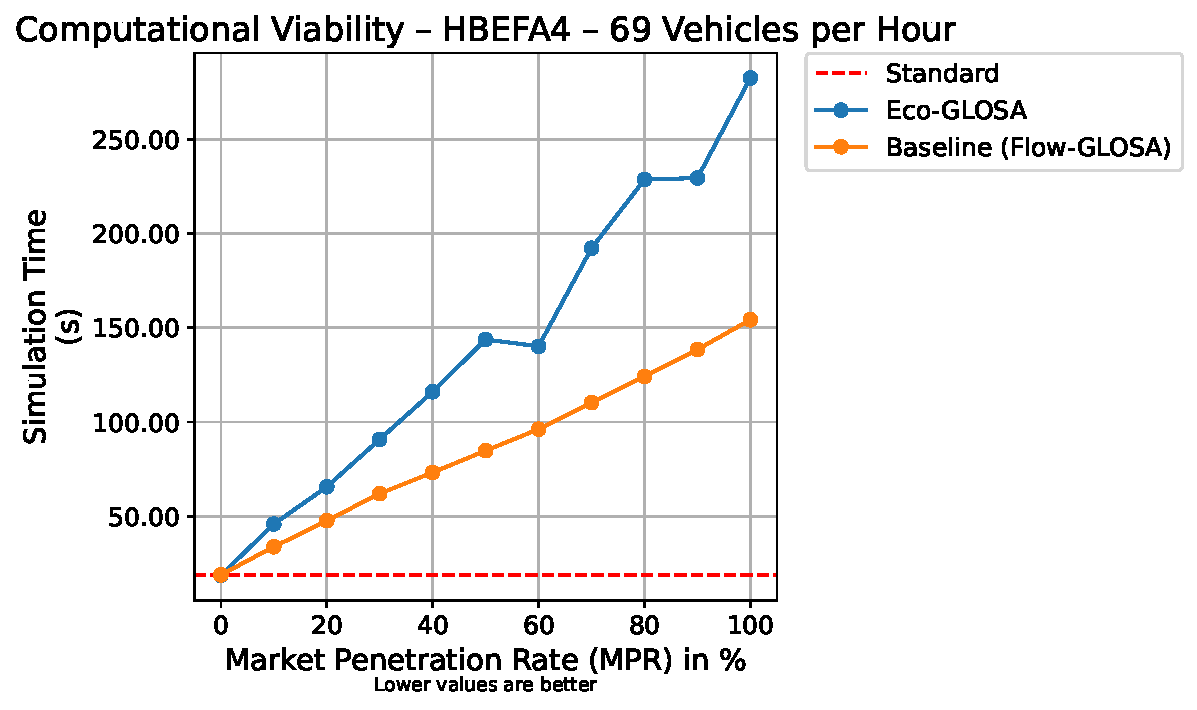
\includegraphics[width=\textwidth]{data/img/ComputationalViability/ComputationalViability_HBEFA4_Cars69.pdf}
    \caption{HBEFA4 at $69\,\mathrm{veh/h}$.}
    \label{fig:Comp_69_HBEFA4}
  \end{subfigure}\hfill
  \begin{subfigure}[b]{0.45\textwidth}
    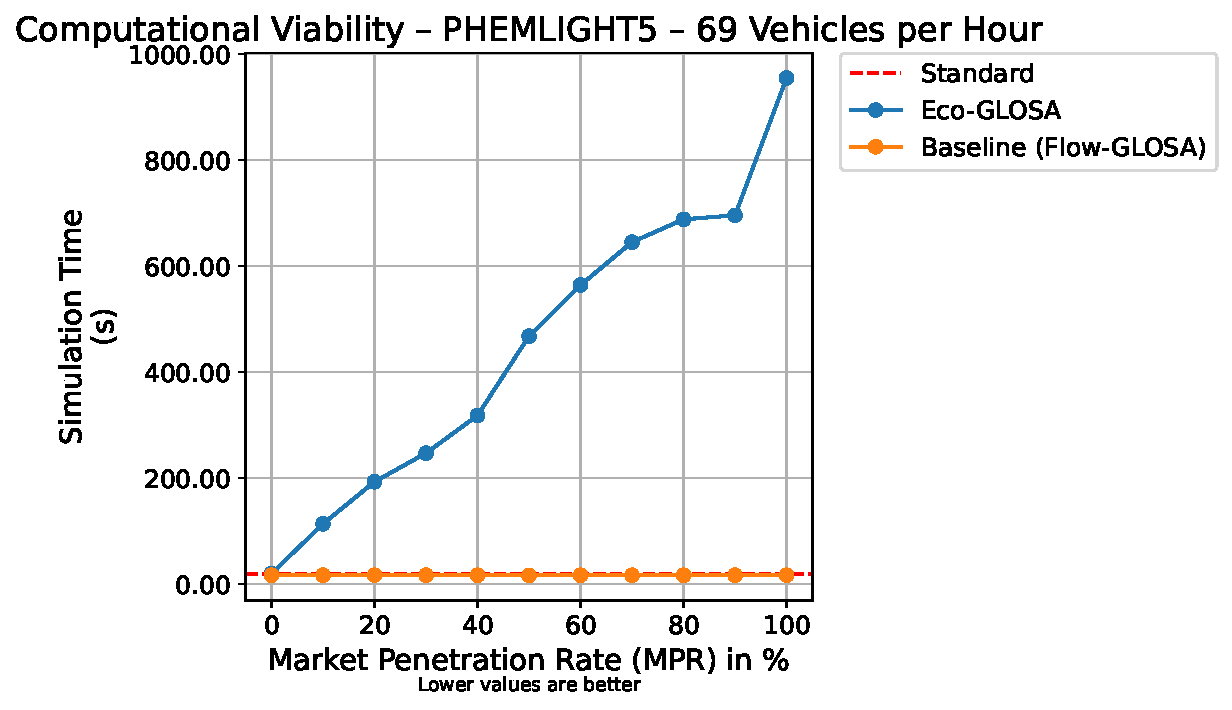
\includegraphics[width=\textwidth]{data/img/ComputationalViability/ComputationalViability_PHEMLIGHT5_Cars69.pdf}
    \caption{PHEMlight5 at $69\,\mathrm{veh/h}$.}
    \label{fig:Comp_69_PHEM}
  \end{subfigure}
  \caption{Simulation time versus \ac{mpr} at low traffic volume.  \ac{eco-glosa} exhibits modest overhead at zero penetration but grows rapidly beyond $50\%$ MPR, especially under PHEMlight5.}
  \label{fig:Comp_69}
\end{figure}

\begin{figure}[htb]
  \centering
  \begin{subfigure}[b]{0.45\textwidth}
    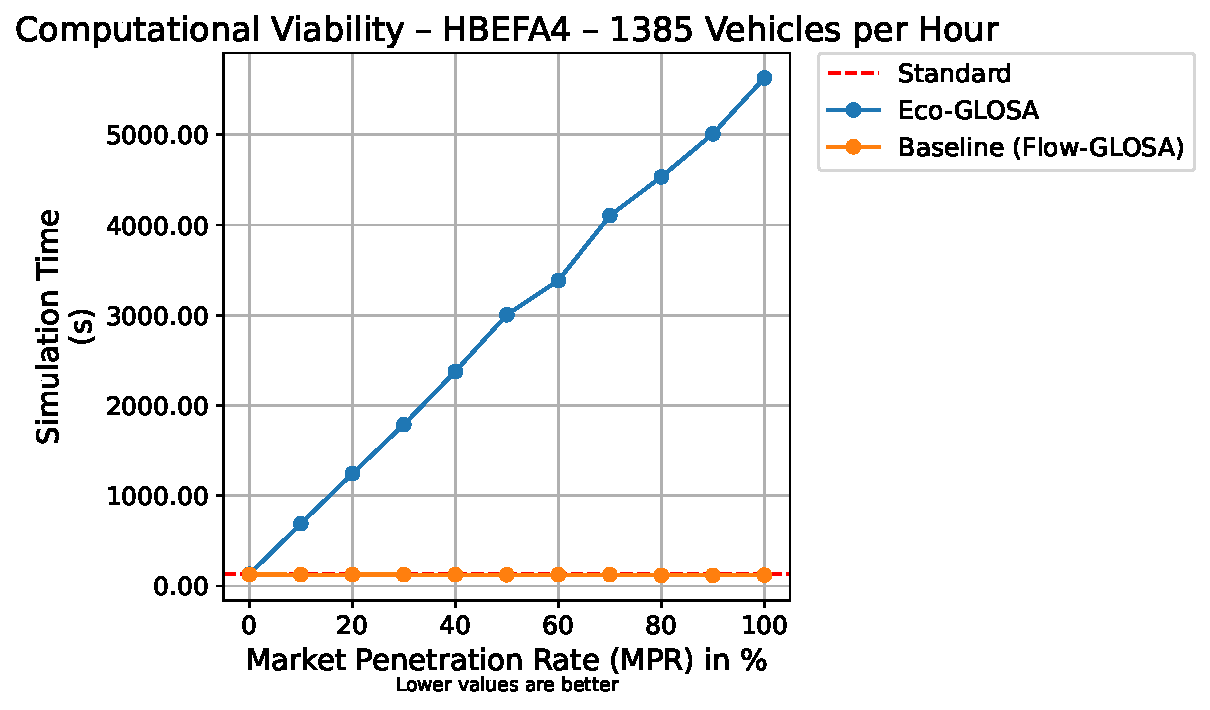
\includegraphics[width=\textwidth]{data/img/ComputationalViability/ComputationalViability_HBEFA4_Cars1385.pdf}
    \caption{HBEFA4 at $1385\,\mathrm{veh/h}$.}
    \label{fig:Comp_1385_HBEFA4}
  \end{subfigure}\hfill
  \begin{subfigure}[b]{0.45\textwidth}
    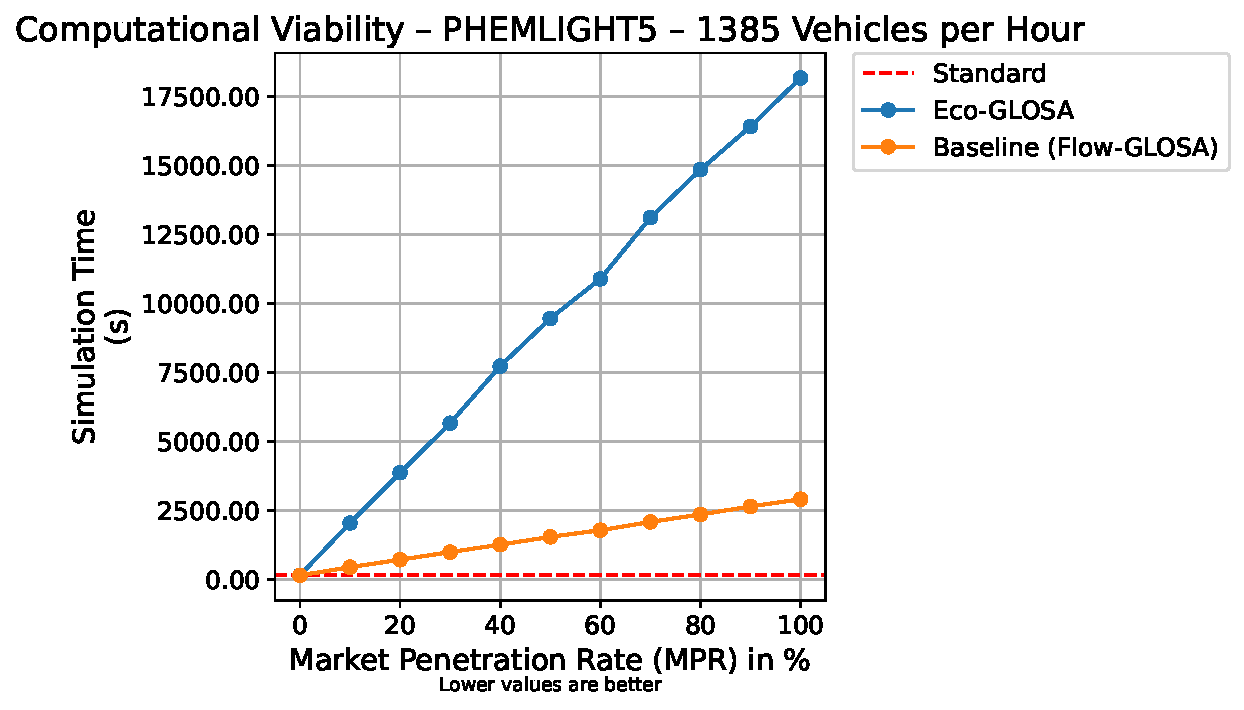
\includegraphics[width=\textwidth]{data/img/ComputationalViability/ComputationalViability_PHEMLIGHT5_Cars1385.pdf}
    \caption{PHEMlight5 at $1385\,\mathrm{veh/h}$.}
    \label{fig:Comp_1385_PHEM}
  \end{subfigure}
  \caption{Simulation time versus \ac{mpr} at intermediate volume.  \ac{eco-glosa} overhead increases from $\sim$1.5$\times$ at 10\% MPR to over 5$\times$ at 100\% MPR compared to \ac{flow-glosa}.}
  \label{fig:Comp_1385}
\end{figure}

\begin{figure}[htb]
  \centering
  \begin{subfigure}[b]{0.45\textwidth}
    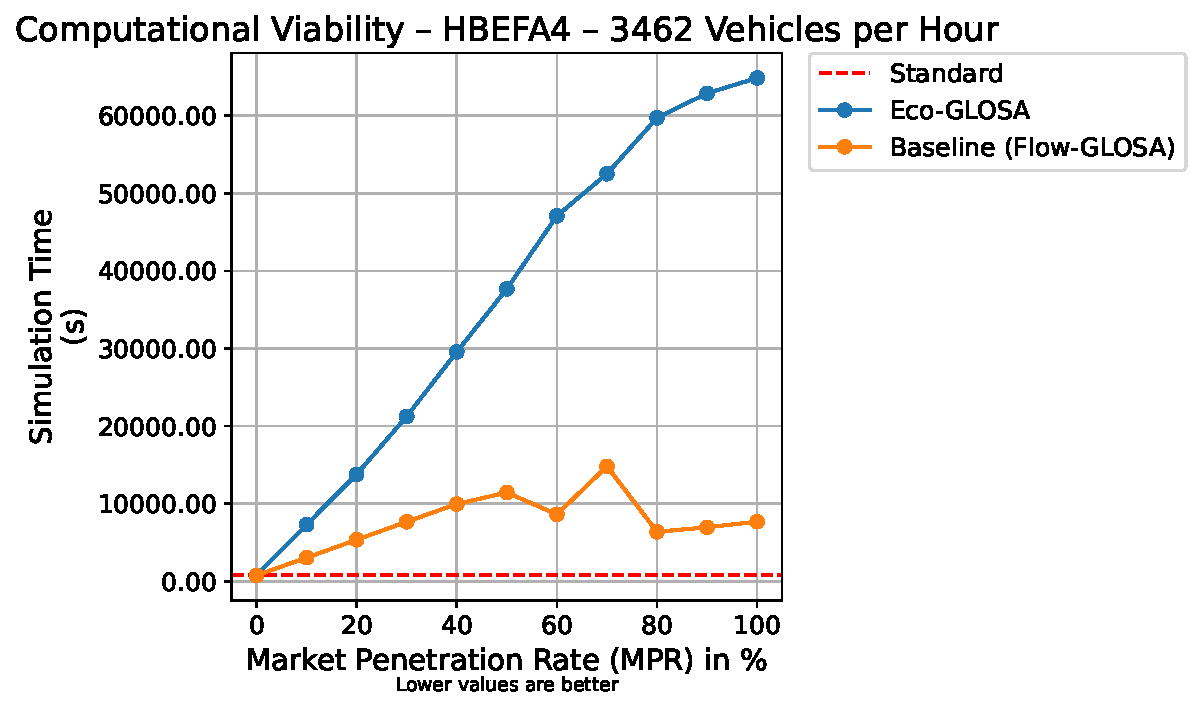
\includegraphics[width=\textwidth]{data/img/ComputationalViability/ComputationalViability_HBEFA4_Cars3462.pdf}
    \caption{HBEFA4 at $3462\,\mathrm{veh/h}$.}
    \label{fig:Comp_3462_HBEFA4}
  \end{subfigure}\hfill
  \begin{subfigure}[b]{0.45\textwidth}
    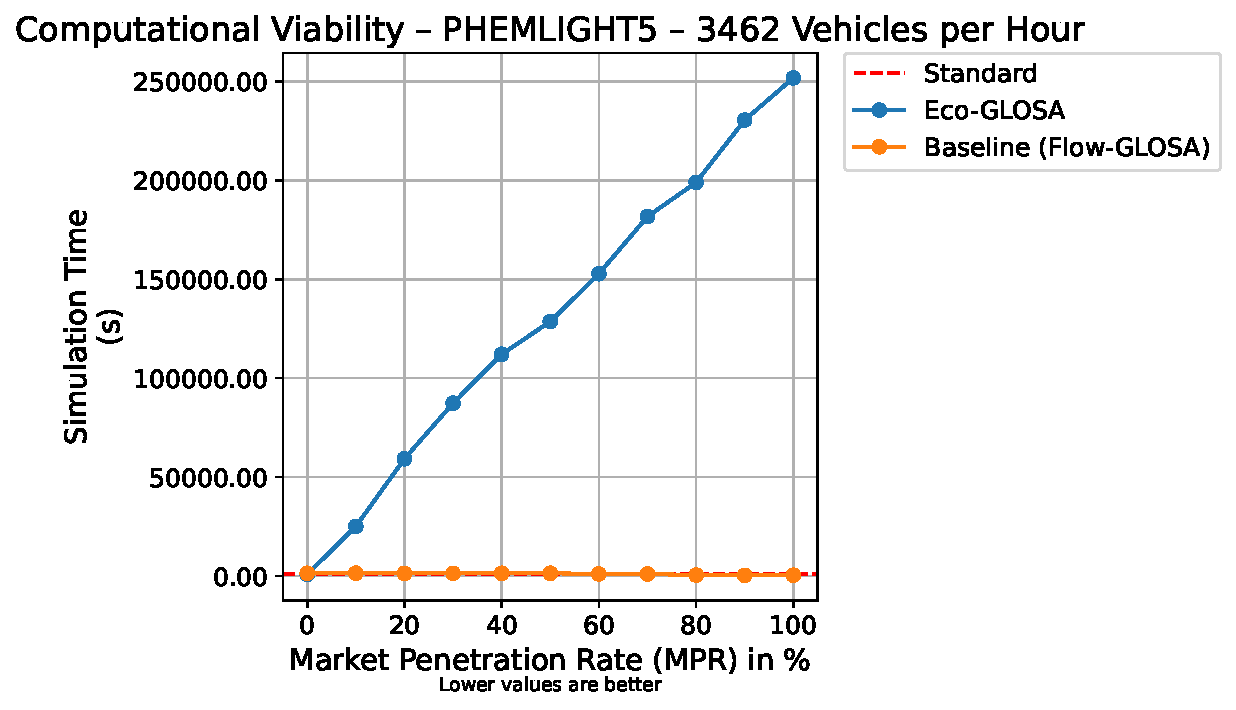
\includegraphics[width=\textwidth]{data/img/ComputationalViability/ComputationalViability_PHEMLIGHT5_Cars3462.pdf}
    \caption{PHEMlight5 at $3462\,\mathrm{veh/h}$.}
    \label{fig:Comp_3462_PHEM}
  \end{subfigure}
  \caption{Simulation time versus \ac{mpr} in the saturated regime.  \ac{eco-glosa} under PHEMlight5 exceeds $250\,000\,$s at full penetration, while \ac{flow-glosa} remains under $8000\,$s.}
  \label{fig:Comp_3462}
\end{figure}

\textbf{In summary}, \ac{eco-glosa} entails a steep computational surcharge, up to $48\times$ slower than the baseline at low volume and more than $30\times$ slower at full saturation under PHEMlight5. The \ac{traci} interface alone imposes an additional $9$–$12\times$ slowdown relative to native \ac{sumo}. These findings underline the necessity of (i) a native or GPU-accelerated \ac{eco-glosa} implementation and (ii) preferring a native \ac{sumo}-based integration over the \ac{traci} interface to minimise communication overhead and achieve practical runtimes in large‐scale or real‐time deployments.

\begin{table}[htb]
  \centering
  \caption{Absolute simulation times of \ac{eco-glosa} and \ac{flow-glosa} implementations under \ac{traci} for various traffic volumes and fuel models. Absolute times depend on hardware and operating system.}
  \label{tab:CompViability_TraciComparison}
  \resizebox{\textwidth}{!}{%
    \begin{tabular}{l l l *{11}{c}}
      \toprule
      Cars & Algorithm                 & Fuel         & \textbf{0\% (Std.)} & 10\%       & 20\%       & 30\%       & 40\%       & 50\%       & 60\%       & 70\%       & 80\%       & 90\%       & 100\%      \\
      \midrule
      69.0  & Eco-GLOSA                  & HBEFA4       & \textbf{18.64}      & 45.85      & 65.61      & 90.83      & 116.07     & 143.79     & 140.17     & 192.22     & 228.63     & 229.47     & 282.56     \\
      69.0  & Baseline (Flow-GLOSA)      & HBEFA4       & \textbf{18.89}      & 33.81 & 47.66      & 62.03      & 73.24      & 84.78      & 96.20      & 110.26     & 124.18     & 138.50     & 154.27     \\
      69.0  & Eco-GLOSA                  & PHEMlight5   & \textbf{19.79}      & 113.47     & 192.99     & 246.83     & 318.11     & 467.78     & 564.11     & 645.15     & 688.17     & 695.72     & \textbf{954.95} \\
      69.0  & Baseline (Flow-GLOSA)      & PHEMlight5   & \textbf{19.74}      & 35.07      & 48.86      & 62.42      & 74.12      & 86.59      & 97.60      & 111.75     & 126.13     & 139.04     & 153.64     \\
      \midrule
      138.0 & Eco-GLOSA                  & HBEFA4       & \textbf{24.35}      & 71.47      & 109.07     & 147.94     & 199.01     & 276.45     & 271.03     & 374.97     & 429.04     & 476.37     & 538.66     \\
      138.0 & Baseline (Flow-GLOSA)      & HBEFA4       & \textbf{24.51}      & 52.91 & 78.94      & 101.98     & 133.92     & 160.74     & 183.96     & 216.30     & 243.30     & 272.53     & 296.83     \\
      138.0 & Eco-GLOSA                  & PHEMlight5   & \textbf{26.35}      & 167.41     & 324.63     & 393.20     & 508.62     & 859.65     & 808.66     & 1041.76    & 1225.48    & 1519.14    & \textbf{1617.62} \\
      138.0 & Baseline (Flow-GLOSA)      & PHEMlight5   & \textbf{26.35}      & 55.08      & 81.36      & 104.24     & 136.92     & 164.67     & 186.48     & 218.25     & 249.58     & 275.22     & 299.86     \\
      \midrule
      346.0 & Eco-GLOSA                  & HBEFA4       & \textbf{41.48}      & 157.89     & 280.45     & 464.09     & 539.94     & 709.78     & 802.68     & 933.80     & 1062.64    & 1178.17    & 1337.18    \\
      346.0 & Baseline (Flow-GLOSA)      & HBEFA4       & \textbf{41.25}      & 108.99 & 179.65     & 253.48     & 309.06     & 382.80     & 449.63     & 510.24     & 581.60     & 654.66     & 697.96     \\
      346.0 & Eco-GLOSA                  & PHEMlight5   & \textbf{45.96}      & 408.26     & 909.13     & 1422.53    & 1636.71    & 2058.14    & 2573.80    & 2762.42    & 3290.75    & 3709.17    & \textbf{4034.62} \\
      346.0 & Baseline (Flow-GLOSA)      & PHEMlight5   & \textbf{45.96}      & 113.87     & 183.71     & 257.67     & 314.50     & 384.77     & 449.25     & 522.51     & 583.57     & 653.83     & 702.11     \\
      \midrule
      692.0 & Eco-GLOSA                  & HBEFA4       & \textbf{70.06}      & 290.22     & 507.57     & 824.96     & 1077.34    & 1316.33    & 1604.01    & 1844.68    & 2081.46    & 2413.43    & 2689.71    \\
      692.0 & Baseline (Flow-GLOSA)      & HBEFA4       & \textbf{70.01}      & 199.61 & 328.83     & 466.43     & 598.32     & 746.09     & 878.61     & 1009.32    & 1138.79    & 1285.82    & 1423.82    \\
      692.0 & Eco-GLOSA                  & PHEMlight5   & \textbf{79.38}      & 830.27     & 1458.45    & 2363.30    & 3059.37    & 3879.64    & 4721.61    & 5316.79    & 6342.07    & 7676.13    & \textbf{8407.14} \\
      692.0 & Baseline (Flow-GLOSA)      & PHEMlight5   & \textbf{78.96}      & 207.93     & 339.90     & 475.03     & 608.61     & 761.29     & 905.29     & 1024.79    & 1159.32    & 1286.28    & 1435.04    \\
      \midrule
      1385.0& Eco-GLOSA                  & HBEFA4       & \textbf{129.28}     & 690.08     & 1243.97    & 1788.03    & 2377.18    & 3004.73    & 3385.14    & 4103.90    & 4533.56    & 5010.08    & 5629.95    \\
      1385.0& Baseline (Flow-GLOSA)      & HBEFA4       & \textbf{129.45}     & 429.51 & 708.63     & 967.43     & 1238.00    & 1535.47    & 1790.18    & 2092.41    & 2322.02    & 2641.07    & 2872.80    \\
      1385.0& Eco-GLOSA                  & PHEMlight5   & \textbf{149.43}     & 2044.34    & 3869.10    & 5660.32    & 7731.41    & 9458.66    & 10890.27   & 13110.24   & 14853.12   & 16414.57   & \textbf{18175.02} \\
      1385.0& Baseline (Flow-GLOSA)      & PHEMlight5   & \textbf{147.99}     & 443.74     & 714.95     & 990.27     & 1261.04    & 1543.80    & 1784.86    & 2084.13    & 2356.39    & 2643.55    & 2908.28    \\
      \midrule
      2077.0& Eco-GLOSA                  & HBEFA4       & \textbf{194.76}     & 1059.69    & 1975.94    & 2762.06    & 3673.14    & 4655.86    & 5286.35    & 6359.72    & 7099.10    & 8021.73    & 8871.25    \\
      2077.0& Baseline (Flow-GLOSA)      & HBEFA4       & \textbf{192.60}     & 627.27 & 1045.43    & 1477.00    & 1903.69    & 2327.89    & 2743.54    & 3146.68    & 3573.26    & 3965.27    & 4393.02    \\
      2077.0& Eco-GLOSA                  & PHEMlight5   & \textbf{226.03}     & 2940.59    & 5345.12    & 8709.82    & 12229.50   & 14562.74   & 17021.70   & 19812.39   & 22670.23   & 24838.64   & \textbf{27842.28} \\
      2077.0& Baseline (Flow-GLOSA)      & PHEMlight5   & \textbf{222.82}     & 652.90     & 1077.84    & 1530.54    & 1937.15    & 2392.21    & 2784.75    & 3172.89    & 3612.89    & 4026.18    & 4391.33    \\
      \midrule
      2769.0& Eco-GLOSA                  & HBEFA4       & \textbf{265.40}     & 1717.59    & 3066.87    & 9783.80 & 9676.92    & 6817.65    & 29119.22 & 9456.50    & 10410.82   & 11515.24   & 12838.56   \\
      2769.0& Baseline (Flow-GLOSA)      & HBEFA4       & \textbf{263.91}     & 911.38     & 1502.86    & 2086.31    & 2665.99    & 3275.49    & 3829.42    & 4361.18    & 4926.63    & 5492.37    & 5976.06    \\
      2769.0& Eco-GLOSA                  & PHEMlight5   & \textbf{306.78}     & 5033.51    & 18916.38   & 47755.69   & 69552.51   & 94654.61   & 114831.96  & 145268.05  & 142126.60  & 165711.80  & \textbf{139171.65} \\
      2769.0& Baseline (Flow-GLOSA)      & PHEMlight5   & \textbf{305.10}     & 944.66     & 1549.56    & 2131.41    & 2691.56    & 3273.49    & 3865.19    & 4369.02    & 4948.13    & 5467.45    & 6036.59    \\
      \midrule
      3462.0& Eco-GLOSA                  & HBEFA4       & \textbf{762.47}     & 7291.92    & 13774.00   & 21248.52   & 29553.07   & 37682.93   & 47089.12   & 52511.10   & 59711.69   & 62882.26   & 64860.61   \\
      3462.0& Baseline (Flow-GLOSA)      & HBEFA4       & \textbf{753.90}     & 3029.19 & 5342.64    & 7660.62    & 9947.82    & 11430.39   & 8613.54    & 14805.14   & 6367.47    & 6947.72    & 7670.32    \\
      3462.0& Eco-GLOSA                  & PHEMlight5   & \textbf{867.03}     & 25083.58   & 59247.59   & 87348.07   & 112061.03  & 128604.77  & 152756.97  & 181628.56  & 198892.38  & 230399.98  & \textbf{251661.36} \\
      3462.0& Baseline (Flow-GLOSA)      & PHEMlight5   & \textbf{858.37}     & 3133.66    & 5465.48    & 7801.65    & 9987.87    & 11538.38   & 8697.48    & 14902.05   & 6354.86    & 7020.78    & 7713.73    \\
      \bottomrule
    \end{tabular}%
  }
\end{table}

\begin{table}[htb]
  \centering
  \caption{Simulation time comparison between native \ac{sumo} and \ac{traci} implementations of \ac{flow-glosa} for low and high traffic scenarios. Absolute durations depend on the computational environment.}
  \label{tab:CompViability_SumoTraci}
  \resizebox{\textwidth}{!}{%
    \begin{tabular}{l l l *{11}{c}}
      \toprule
      Cars & Interface    & Fuel         & \textbf{0\% (Std.)} & 10\%       & 20\%       & 30\%       & 40\%       & 50\%       & 60\%       & 70\%       & 80\%       & 90\%       & 100\%      \\
      \midrule
      69.0  & \ac{sumo}     & HBEFA4       & \textbf{15.51}      & 15.38      & 15.64      & 15.55      & 15.52      & 15.79      & 15.15      & 15.41      & 15.52      & 15.31      & \textbf{15.20}      \\
      69.0  & \ac{traci}    & HBEFA4       & \textbf{18.89}      & \textbf{33.81} & 47.66      & 62.03      & 73.24      & 84.78      & 96.20      & 110.26     & 124.18     & 138.50     & \textbf{154.27}     \\
      69.0  & \ac{sumo}     & PHEMlight5   & \textbf{16.47}      & 16.34      & 16.41      & 16.61      & 16.47      & 15.98      & 16.39      & 16.24      & 16.37      & 16.37      & \textbf{16.42}      \\
      69.0  & \ac{traci}    & PHEMlight5   & \textbf{19.74}      & \textbf{35.07} & 48.86      & 62.42      & 74.12      & 86.59      & 97.60      & 111.75     & 126.13     & 139.04     & \textbf{153.64}     \\
      \midrule
      3462.0& \ac{sumo}     & HBEFA4       & \textbf{732.46}     & 738.94     & 744.20     & 696.91     & 713.94     & 729.21     & 709.81     & 686.57     & 739.10     & 725.49     & \textbf{727.38}     \\
      3462.0& \ac{traci}    & HBEFA4       & \textbf{753.90}     & \textbf{3029.19} & 5342.64    & 7660.62    & 9947.82    & 11430.39   & 8613.54    & 14805.14   & 6367.47    & 6947.72    & \textbf{7670.32}    \\
      3462.0& \ac{sumo}     & PHEMlight5   & \textbf{834.27}     & 842.27     & 848.58     & 792.96     & 819.15     & 832.40     & 815.79     & 785.65     & 846.47     & 835.91     & \textbf{831.79}     \\
      3462.0& \ac{traci}    & PHEMlight5   & \textbf{858.37}     & \textbf{3133.66} & 5465.48    & 7801.65    & 9987.87    & 11538.38   & 8697.48    & 14902.05   & 6354.86    & 7020.78    & \textbf{7713.73}    \\
      \bottomrule
    \end{tabular}%
  }
\end{table}